\section{案例研究}
% \section{Case Studies}
\label{sec:case-studies}

% This section relates three independently-developed, published projects from diverse domains
%   that incorporated \egg
%   as an easy-to-use, high-performance \egraph implementation.
% In all three cases, the developers had first rolled their own \egraph
%   implementations.
% \Egg allowed them to delete code, gain performance, and in some cases
%   dramatically broaden the project's scope thanks to \egg's speed and
%   flexibility.
% In addition to gaining performance, all three projects use \egg's novel
%   extensibility features like \eclass analyses and dynamic/conditional rewrites.
本节介绍了三个独立开发的、来自不同领域的公开项目,
  它们将 \egg 作为一种易用的、高性能的 \egraph 实现。
在所有这三个案例中,开发者首先推出了他们自己的 \egraph 实现。
由于 \egg 的速度和灵活性,他们可以删除代码,获得性能,并在某些情况下极大地扩大了项目的范围。
除了获得性能外,这三个项目都使用了 \egg 的新颖的可扩展性特性,如 \eclass 分析和动态/条件重写。


% \subsection{Herbie: Improving Floating Point Accuracy}
\subsection{Herbie:提高浮点精度}
\label{sec:herbie}


% Herbie automatically improves accuracy
%   for floating-point expressions,
%   using random sampling to measure error,
%   a set of rewrite rules for generating program variants,
%   and algorithms that prune and combine program variants
%   to achieve minimal error.
% Herbie received PLDI 2015's Distinguished Paper award~\cite{herbie}
%   and has been continuously developed since then,
%   sporting hundreds of Github stars, hundreds of downloads,
%   and thousands of users on its online version.
% Herbie uses \egraphs for algebraic simplification of mathematical expressions,
%   which is especially important for avoiding floating-point errors
%   introduced by cancellation, function inverses, and redundant computation.
Herbie 自动提高了浮点表达式的准确性,使用随机抽样来测量误差,
  使用一套重写规则来生成程序变体,并使用算法来修剪和组合程序变体以达到最小误差。
Herbie 获得了 PLDI 2015 的杰出论文奖~\cite{herbie}。从那时起,Herbie 一直在不断发展。
  在Github上获得了数以百计的 star 和下载量,在其在线版本上有成千上万的用户。
Herbie 使用 \egraphs 对数学表达式进行代数简化,
  这对于避免由消解(cancellation)、函数反转(function inverses) % ?
  和冗余计算(redundant computation)引入的浮点错误尤为重要。 % ?


% Until our case study,
%   Herbie used a custom \egraph implementation
%   written in Racket (Herbie's implementation language)
%   that closely followed traditional \egraph implementations.
% With timeouts disabled,
%   \egraph-based simplification consumed
%   the vast majority of Herbie's run time.
% As a fix, Herbie sharply limits the simplification process,
%   placing a size limit on the \egraph itself and a time limit on the whole
%   procedure.
% When the timeout is exceeded, simplification fails altogether.
% Furthermore, the Herbie authors knew of several features
%   that they believed would improve Herbie's output
%   but could not be implemented because
%   they required more calls to simplification
%   and would thus introduce unacceptable slowdowns.
% Taken together, slow simplification reduced Herbie's performance, completeness,
%   and efficacy.
在我们的案例研究之前,
  Herbie 使用了一个用 Racket(Herbie 的实现语言)编写的定制的 \egraph 实现,
  它紧跟传统的 \egraph 实现。
在禁用超时的情况下,
  基于 \egraph 的简化工作消耗了 Herbie 的绝大部分运行时间。
作为一种修正,Herbie 对简化过程进行了严格的限制,
  对 \egraph 本身设置了大小限制,对整个过程设置了时间限制。
当超过时间限制时,简化过程就会完全失败。
此外,Herbie 的作者还知道一些他们认为可以改善 Herbie 输出的功能,
  但却无法实现,因为它们需要更多的简化调用,因此会带来不可接受的减速。
总的来说,缓慢的简化过程降低了 Herbie 的性能、完整性和有效性。


% We implemented a \egg simplification backend for Herbie.
% The \egg backend is over $3000\times$ faster than Herbie's initial simplifier and
%   is now used by default as of Herbie 1.4.
% Herbie has also backported some of \egg's features like batch simplification and
%   rebuilding to its \egraph implementation
%   (which is still usable, just not the default),
%   demonstrating the portability of \egg's conceptual improvements.
% % This has led to over a $200\times$ speedup over its initial design,
% %   demonstrating that \egg's
我们为Herbie实现了一个egg简化的后端。
\egg 后端比 Herbie 的初始简化器快 $3000\times$,现在已被 Herbie 1.4 已经默认使用。
Herbie 还将一些 \egg 的功能,如批量简化和重建移植到它的 \egraph 实现中
  (它仍然可用,只是不是默认的),证明了 \egg 的概念改进的可移植性。


% \subsubsection{Implementation}
\subsubsection{实现}

% Herbie is implemented in Racket while \egg is in Rust;
%   the \egg simplification backend is thus implemented as a Rust library that
%   provides a C-level API for Herbie to access via foreign-function interface (FFI).
% The Rust library defines the Herbie expression grammar
%   (with named constants, numeric constants, variables, and operations)
%   as well as the \eclass analysis necessary to do constant folding.
% The library is implemented in under 500 lines of Rust.
Herbie 用 Racket 实现,而 \egg 用 Rust 实现;
  因此 \egg 的简化后端被实现为一个 Rust 库,
  提供一个 C 级 API,供 Herbie 通过外部函数接口 (FFI) 访问。
Rust 库定义了 Herbie 表达式语法(带有命名常量、数值常量、变量和操作),
  以及进行常量折叠所需的 \eclass 分析。
该库用不到 500 行的 Rust 代码实现。

% Herbie's set of rewrite rules is not fixed;
%   users can select which rewrites to use using command-line flags.
% Herbie serializes the rewrites to strings,
%   and the \egg backend parses and instantiates them on the Rust side.
Herbie 的重写规则集并不固定;用户可以使用命令行标志来选择使用哪些重写。
Herbie 将重写规则序列化为字符串,而 EGG 后端则在 Rust 端解析并实例化它们。

% Herbie separates exact and inexact program constants:
%   exact operations on exact constants
%   (such as the addition of two rational numbers)
%   are evaluated and added to the \egraph,
%   while operations on inexact constants or that yield inexact outputs
%   are not.
% We thus split numeric constants in the Rust-side grammar
%   between exact rational numbers and inexact constants,
%   which are described by an opaque identifier,
%   and transformed Racket-side expressions into this form
%   before serializing them and passing them to the Rust driver.
Herbie 分离了精确和不精确的程序常量:
  对精确常量的精确操作(如两个有理数的加法)会被评估并添加到 \egraph 中,
  而对不精确常量或产生不精确输出的操作则不会。
因此,我们将 Rust 端语法中的数字常量分为精确的有理数和不精确的常量,
  它们由一个不透明的标识符(opaque identifier)描述,
  并将 Racket 端表达式转化为这种形式,
  然后将它们序列化并传递给 Rust 驱动。
% To evaluate operations on exact constants,
%   we used the constant folding \eclass analysis
%   to track the ``exact value'' of each \eclass.%
% \footnote{Herbie's rewrite rules guarantee that different exact values
%   can never become equal; the semilattice \textsf{join} checks this invariant on the Rust side.}
% Every time an operation \enode is added to the \egg \egraph,
%   we check whether all arguments to that operation have exact value (using the analysis data),
%   and if so do rational number arithmetic to evaluate it.
% The \eclass analysis is cleaner than the corresponding code in Herbie's implementation,
%   which is a built-in pass over the entire \egraph.
为了评估精确常量上的操作,
  我们使用了常量折叠的 \eclass 分析来跟踪每个 \eclass 的“精确值”。
  \footnote{ Herbie 的重写规则保证了不同的精确值永远不能变得相等;
  半格 \textsf{加入}(semilattice \textsf{join})在 Rust 端检查这个不变量。 % ?
  }
每当一个运算符 \enode 被添加到 \egg \egraph 时,
  我们会检查该操作的所有参数是否具有精确值(使用分析的数据),
  如果是则进行有理数运算去计算它。
\eclass 分析比 Herbie 实现中相应的代码更干净,
  因为它是整个 \egraph 的内建过程(built-in pass)。 % ? over

% \subsubsection{Results}
\subsubsection{评估}

\begin{figure}
  \centering
  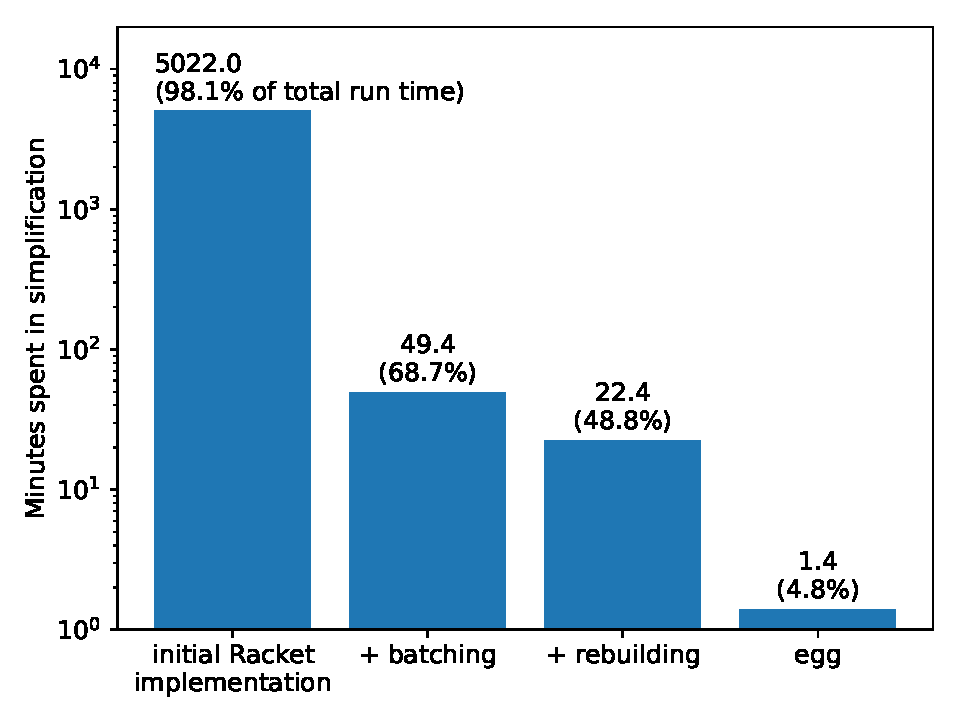
\includegraphics[height=5.5cm]{herbie}
  \caption{
    % Herbie sped up its expression simplification phase
    %   by adopting \egg-inspired features like
    %   batched simplification and rebuilding
    %   into its Racket-based \egraph implementation.
    % Herbie also supports using \egg itself for additional speedup.
    % Note that the y-axis is log-scale.
    Herbie 通过在 基于 Racket 的 \egraph 实现中采用像批量简化和重建这样的 \egg 启发式特性,% ?
      来加速其表达式简化阶段。
    Herbie 还支持使用 \egg 本身来获得额外的加速。
    注意 y 轴是对数刻度。
  }
  \label{fig:herbie-results}
\end{figure}


% Our \egg simplification backend
%   is a drop-in replacement to the existing Herbie simplifier,
%   making it easy to compare speed and results.
% We compare using
%   Herbie's standard test suite of roughly 500 benchmarks,
%   with timeouts disabled.
% \autoref{fig:herbie-results} shows the results.
% The \egg simplification backend is over
%   $3000\times$ faster than Herbie's initial simplifier.
% This speedup eliminated Herbie's largest bottleneck:
%   the initial implementation dominated Herbie's total run time at $98.1\%$,
%   backporting \egg improvements into Herbie cuts
%   that to about half the total run time,
%   and \egg simplification takes under $5\%$ of the total run time.
% Practically, the run time of Herbie's initial implementation was smaller, since
%   timeouts cause tests failures when simplification takes too long.
% Therefore, the speedup also improved Herbie's completeness,
%   as simplification now never times out.
\egg 简化器后端是现有 Herbie 简化器的插入式替代品(drop-in replacement),
  使比较速度和结果变得容易。
我们使用 Herbie 的标准测试套件,大约有500个基准测试,其中禁用了超时。
\autoref{fig:herbie-results} 显示了测试结果。
\egg 简化后端比 Herbie 的初始简化器快了 $3000\times$。
这种加速消除了 Herbie 的最大瓶颈:
  原始实现占 Herbie 总运行时间的 $98.1\%$,
  将 \egg 改进移植到 Herbie 中将其减少到总运行时间的一半,
  \egg 简化器占总运行时间的不到 $5\%$ 。
实际上,Herbie 初始实现的运行时间更短,因为超时会导致简化时间过长时测试失败。
因此加速也提高了 Herbie 的完备性,因为简化过程现在永远不会超时,。


% Since incorporating \egg into Herbie, the Herbie developers have backported some
%   of \egg's key performance improvements into the Racket \egraph implementation.
% First, batch simplification gives a large speedup because Herbie simplifies many
%   similar expressions.
% When done simultaneously in one equality saturation, the \egraph's structural
%   sharing can massively deduplicate work.
% Second, deferring rebuilding (as discussed in \autoref{sec:rebuilding}) gives a
%   further $2.2\times$ speedup.
% As demonstrated in \autoref{fig:eval-iter}, rebuilding offers an asymptotic
%   speedup, so Herbie's improved implementation (and the \egg backend as well)
%   will scale better as the search size grows.
自从将 \egg 纳入 Herbie 以来,Herbie 开发人员已经将一些
  \egg 的关键性能改进移植到了 Racket \egraph 实现中。
首先,批量简化给出了很大的加速,因为 Herbie 简化了许多相似的表达式。
在一个 等式饱和 的同时进行时,\egraph 的结构共享可以大量地减少重复工作。
其次,推迟重建 (如 \autoref{sec:rebuilding} 中所述) 给出了进一步的 $2.2\times$ 加速。
如 \autoref{fig:eval-iter} 所示,重建提供了渐近
  加速,因此 Herbie 的改进实现 (以及 \egg 后端)
  将随着搜索规模的增长而更好地扩展(scale)。 % ?scale

% \subsection{Spores: Optimizing Linear Algebra}
\subsection{Spores: 优化线性代数}
\label{sec:spores}


% Spores \cite{spores} is an optimizer for machine learning programs. It
% translates linear algebra (LA) expressions to relational algebra (RA), performs
% rewrites, and finally translates the result back to linear algebra. Each rewrite
% is built up from simple identities in relational algebra like the associativity
% of join. These relational identities express more fine-grained equality than
% textbook linear algebra identities, allowing Spores to discover novel
% optimizations not found by traditional optimizers based on LA identities. Spores
% performs holistic optimization, taking into account the complex interactions
% among factors like sparsity, common subexpressions, and fusible operators and
% their impact on execution time.
Spores \cite{spores} 是一个机器学习程序的优化器。
它将线性代数(LA)表达式翻译成关系代数(RA),进行重写,最后将结果再翻译成线性代数。
每一次重写都是由关系代数中的简单特性建立起来的,比如连接的关联性。
与教科书上的线性代数特性相比,这些关系特性表达了更精细的平等性,
使得 Spores 能够发现传统优化器基于 LA 特性所不能发现的新型优化。
Spores 进行整体优化(holistic optimization),
考虑到诸如稀疏性、共同子表达式和可融合运算符等因素之间复杂的相互作用以及它们对执行时间的影响。


% \Max{we should probably tone down some of the language below}

% \subsubsection{Implementation}
\subsubsection{实现}
% \Max{don't say ``we''}


% Spores is implemented entirely in Rust using \Egg.
% \Egg empowers Spores to orchestrate
%   the complex interactions described above elegantly and effortlessly.
% Spores works in three steps: first, it translates the input LA expression to RA;
% second, it optimizes the RA expression by equality saturation; finally, it
% translates the optimized RA expression back to LA.
Spores 完全用 Rust 和 \Egg 实现。
\Egg 赋予 Spores 优雅而轻松地编排上述复杂交互。
Spores 工作三个步骤:首先,它将输入的 LA 表达式转换为 RA;
其次,它通过 等式饱和 优化 RA 表达式;最后,它
将优化后的 RA 表达式转换回 LA。
% Since the translation between LA and RA is
% straightforward, we focus the discussion on the equality saturation step in RA.
% Spores represents a relation as a function from tuples to real numbers: $A:
% (a_1, a_2, ..., a_n) \rightarrow \mathbb{R}$. This is similar to the index
% notation in linear algebra, where a matrix A can be viewed as a function
% $\lambda i, j . A_{ij}$. A tuple is identified with a named record,
% e.g. $(1, 2) = \{a_1: 1, a_2: 2\} = \{a_2: 2, a_1: 1\}$, so that order in a
% tuple doesn't matter. There are just three operations on relations: join, union
% and aggregate. Join ($\otimes$) takes two relations and returns their natural
% join, multiplying the associated real number for joined tuples:
由于 LA 和 RA 之间的转换是直接的,因此我们将讨论集中在 RA 中的 等式饱和 步骤上。
Spores 将关系表示为从元组到实数的函数: 
$A: (a_1, a_2, ..., a_n) \rightarrow \mathbb{R}$。
这类似于线性代数中的索引符号,其中矩阵 A 可以被视为函数 
$\lambda i, j . A_{ij}$。
元组与命名记录相同,例如 $(1, 2) = \{a_1: 1, a_2: 2\} = \{a_2: 2, a_1: 1\}$,
因此元组中的顺序无关紧要。关系上只有三种操作: join, union 和 aggregate。 
Join ($\otimes$) 接受两个关系并返回它们的自然 join,将连接元组的关联实数相乘:
\[ A \otimes B = \lambda \bar{a} \cup \bar{b} . A(\bar{a}) \times B(\bar{b})\]
% 此段翻译未仔细校对
% Here $\bar{a}$ is the set of field names for the records in $A$. In RA
% terminology, $\bar{a}$ is the {\em schema} of $A$. Union ($\oplus$) is a join in
% disguise: it also performs natural join on its two arguments, but adds the
% associated real instead of multiplying it:
这里 $\bar{a}$ 是 $A$ 中记录的字段名集合。
在 RA 术语中,$\bar{a}$ 是 $A$ 的 {\em schema}。
Union ($\oplus$) 是一种伪装的 join:它在其两个参数上也执行自然 join,但是添加而不是乘以关联实数:
\[A \oplus B = \lambda \bar{a} \cup \bar{b} . A(\bar{a}) + B(\bar{b})\] 
% Finally, aggregate ($\Sigma$) sums its argument along a given dimension. It
% coincides precisely with the ``sigma notation'' in mathematics:
最后, aggregate($\Sigma$) 沿给定维度求和其参数。它与数学中的“sigma 符号”完全相同:
\[\sum_{a_i} A = \lambda \bar{a}-a_i . \sum_{a_i} A(\bar{a})\]

% \begin{figure}
% \centering
% \begin{align}
%   \label{eq:RRC_pp} A \oplus (B \oplus C) &= \oplus (A, B, C)
%   & \text{($\oplus$ is assoc. \& comm.)}
%   \\
%   \label{eq:RRC_mm} A \otimes (B \otimes C) &= \otimes (A, B, C)
%   & \text{($\otimes$ is assoc. \& comm.)}
%   \\
%   \label{eq:RRC_mp} A \otimes (B \oplus C) &= A \otimes B \oplus A \otimes C
%   & \text{($\otimes$ distributes over $\oplus$)}
%   \\
%   \label{eq:RRC_ap} \sum_i (A \oplus B) &= \sum_i A \oplus \sum_i B
%   \\
%   \label{eq:RRC_aa} \sum_i \sum_j A &= \sum_{i,j} A
%   \\
%   \label{eq:RRC_ma} A \otimes \sum_i B &= \sum_i (A \otimes B)
%   &\text{(requires $i \not\in A$)}
%   \\
%   \label{eq:RRC_ac} \sum_i A &= A \otimes \textsf{dimension}(i)
%   &\text{(requires $i \not\in A$)}
% \end{align}
% % \caption{RA equality rules $R_{EQ}$.}
% \caption{RA 等式规则~$R_{EQ}$.}
% \label{fig:RRC}
% \end{figure}
\begin{figure}
\centering
\begin{align}
  \label{eq:RRC_pp} A \oplus (B \oplus C) &= \oplus (A, B, C)
  & \text{($\oplus$ 满足结合律 \& 交换律)}
  \\
  \label{eq:RRC_mm} A \otimes (B \otimes C) &= \otimes (A, B, C)
  & \text{($\otimes$ 满足结合律 \& 交换律)}
  \\
  \label{eq:RRC_mp} A \otimes (B \oplus C) &= A \otimes B \oplus A \otimes C
  & \text{($\otimes$ 对于 $\oplus$ 满足分配率)}
  \\
  \label{eq:RRC_ap} \sum_i (A \oplus B) &= \sum_i A \oplus \sum_i B
  \\
  \label{eq:RRC_aa} \sum_i \sum_j A &= \sum_{i,j} A
  \\
  \label{eq:RRC_ma} A \otimes \sum_i B &= \sum_i (A \otimes B)
  &\text{(要求 $i \not\in A$)}
  \\
  \label{eq:RRC_ac} \sum_i A &= A \otimes \textsf{dimension}(i)
  &\text{(要求 $i \not\in A$)}
\end{align}
% \caption{RA equality rules $R_{EQ}$.}
\caption{RA 等式规则 $R_{EQ}$.}
\label{fig:RRC}
\end{figure}


% 此段翻译未仔细校对
% The RA identities, presented in \autoref{fig:RRC}, are also simple and intuitive.
% The notation $i \not\in A$ means $i$ is not in the schema of $A$, and $dim(i)$
% is the size of dimension $i$ (e.g. length of rows in a matrix). In
% \autoref{eq:RRC_ma}, when $i \in A$, we first rename every $i$ to a fresh variable
% $i'$ in $B$, which gives us: $A \otimes \sum_i B = \sum_{i'} (A \otimes B[i
% \rightarrow i'])$. In addition to these equalities, Spores also supports
% replacing expressions with fused operators. For example, $(X-UV)^2$ can be
% replaced by $sqloss(X, U, V)$ which streams values from $X, U, V$ and
% computes the result without creating intermediate matrices. Each of these fused
% operators is encoded with a simple identity in \Egg.
在 \autoref{fig:RRC} 中呈现的 RA 指示器(identities)也是简单直观的。 %?RA identities
符号$i \not\in A$ 表示 $i$ 不在 $A$ 的模式中,
  $dim(i)$ 是维度 $i$ 的大小(例如,矩阵中的行长度)。
在\autoref{eq:RRC_ma} 中,当$i \in A$ 时,我们首先将$i$重命名为$B$中的新变量$i'$,
  这给我们:$A \otimes \sum_i B = \sum_{i'} (A \otimes B[i \rightarrow i'])$。
除了这些等式之外,Spores 还支持用融合运算符替换表达式。
例如,$(X-UV)^2$ 可以用 $sqloss(X, U, V)$ 替换,
这将从 $X, U, V$ 中流式传输值并在不创建中间矩阵的情况下计算结果。
这些融合运算符中的每一个都在 \Egg 中以简单身份编码。

% 此段翻译未仔细校对
% Note that \autoref{eq:RRC_ma} requires a way
% to store the schema of every expression during optimization.
% Spores uses an \eclass analysis to annotate \eclasses with the appropriate
%   schema. It also leverages the \eclass analysis for cost estimation,
%   using a conservative cost model that overapproximates.
% As a result, equivalent expressions may have different cost estimates.
% The \texttt{merge} operation on the analysis data takes the lower cost,
%   incrementally improving the cost estimate.
% Finally, Spores' \eclass analysis also performs constant folding.
% As a whole, the \eclass analysis is a composition of three smaller analyses
%   in a similar style to the composition of lattices in abstract interpretation.
注意,在优化过程中,\autoref{eq:RRC_ma} 需要存储每个表达式的模式。
Spores 使用 \eclass 分析来为 \eclasses 注释适当的模式,
  它还利用\eclass 分析进行成本估算,使用过高估计的保守成本模型。
因此,等价的表达式可能具有不同的成本估计。
  对分析数据的 \texttt{merge} 操作采用较低的成本,逐渐改善成本估计。
最后,Spores的 \eclass 分析还执行常量折叠。
总之,\eclass 分析是三个较小分析的组合,
  类似于抽象解释中的格点(lattices)组合。% ? composition of lattices

% \subsubsection{Results}
\subsubsection{评估}

% Spores is integrated into Apache SystemML \cite{Boehm_2019} in a prototype,
% where it is able to derive all of 84 hand-written rules and heuristics for
% sum-product optimization. It also discovered novel rewrites that contribute
% to $1.2\times$ to $5\times$ speedup in end-to-end experiments. With greedy
% extraction, all compilations completed within a second.
Spores 已被集成到 Apache SystemML \cite{Boehm_2019} 的原型中,
在那里它能够推导出 84 个手写的规则(hand-written rules)和启发式算法来进行和积优化。
它还发现了新的重写,在端到端实验中贡献了 $1.2\times$ 到 $5\times$ 的加速。
使用贪心提取(greedy extraction),所有编译能都在一秒钟内完成。 %?greedy extraction


% \subsection{Szalinski: Decompiling CAD into Structured Programs}
\subsection{Szalinski: 将 CAD 反编译为结构化程序}
\label{sec:szalinski}

% \begin{figure}
%   \centering
%   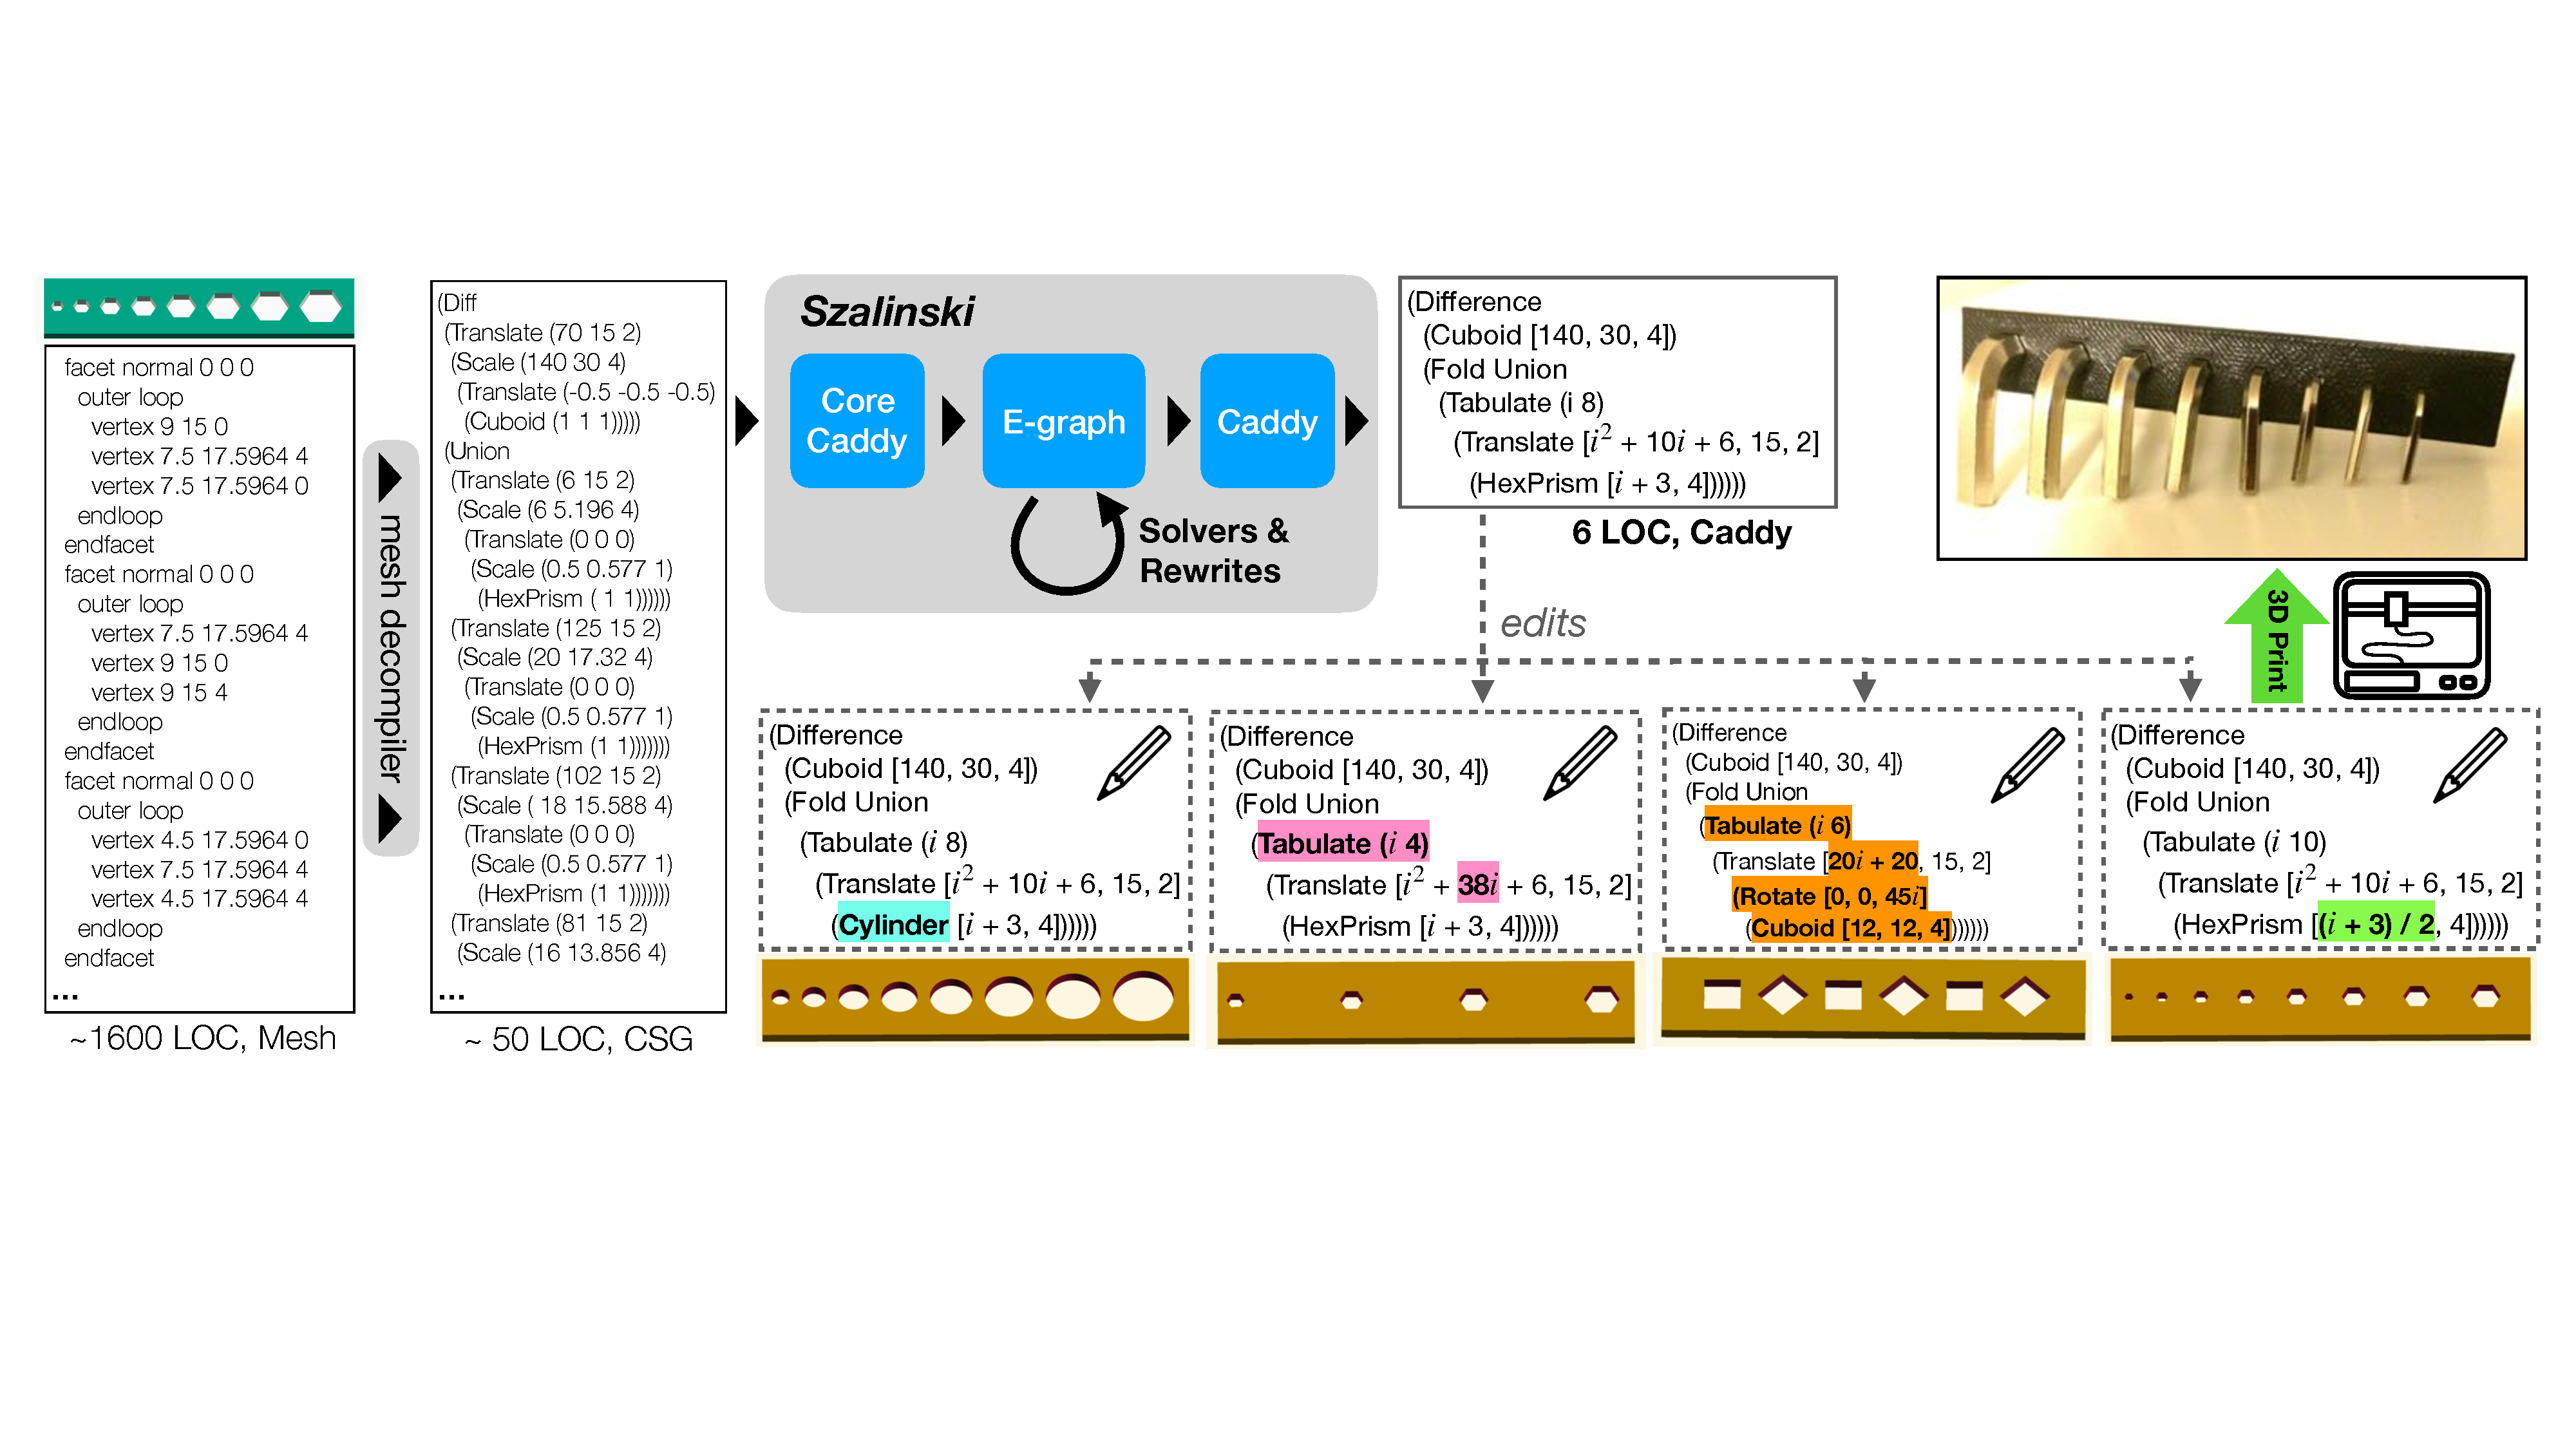
\includegraphics[width=\linewidth]{sz-overview}
%   \caption[Szalinski decompiles flat CSG into structured CAD]{
%   (Figure from Nandi et.\ al.\ \cite{szalinski})
%   Existing mesh decompilers turn
%     triangle meshes into flat, computational solid geometry (CSG) expressions.
%   %  The size of both mesh and CSG are roughly proportional to
%   %    the number of geometric features in the CAD model.
%   \sz~\cite{szalinski} takes in these CSG expressions
%     in a format called Core Caddy,
%     and it synthesizes smaller, structured programs in language called Caddy
%     that is enriched with functional-style features.
%   This can ease customization by simplifying edits:
%     small, mostly local changes
%     yield usefully different models.
%   The photo shows the 3D printed hex wrench holder after
%     customizing hole sizes.
%   \sz is powered by \egg's extensible equality saturation, relying on its high
%     performance, \eclass analyses, and dynamic rewrites.
%   }
%   \label{fig:sz-overview}
% \end{figure}
\begin{figure}
  \centering
  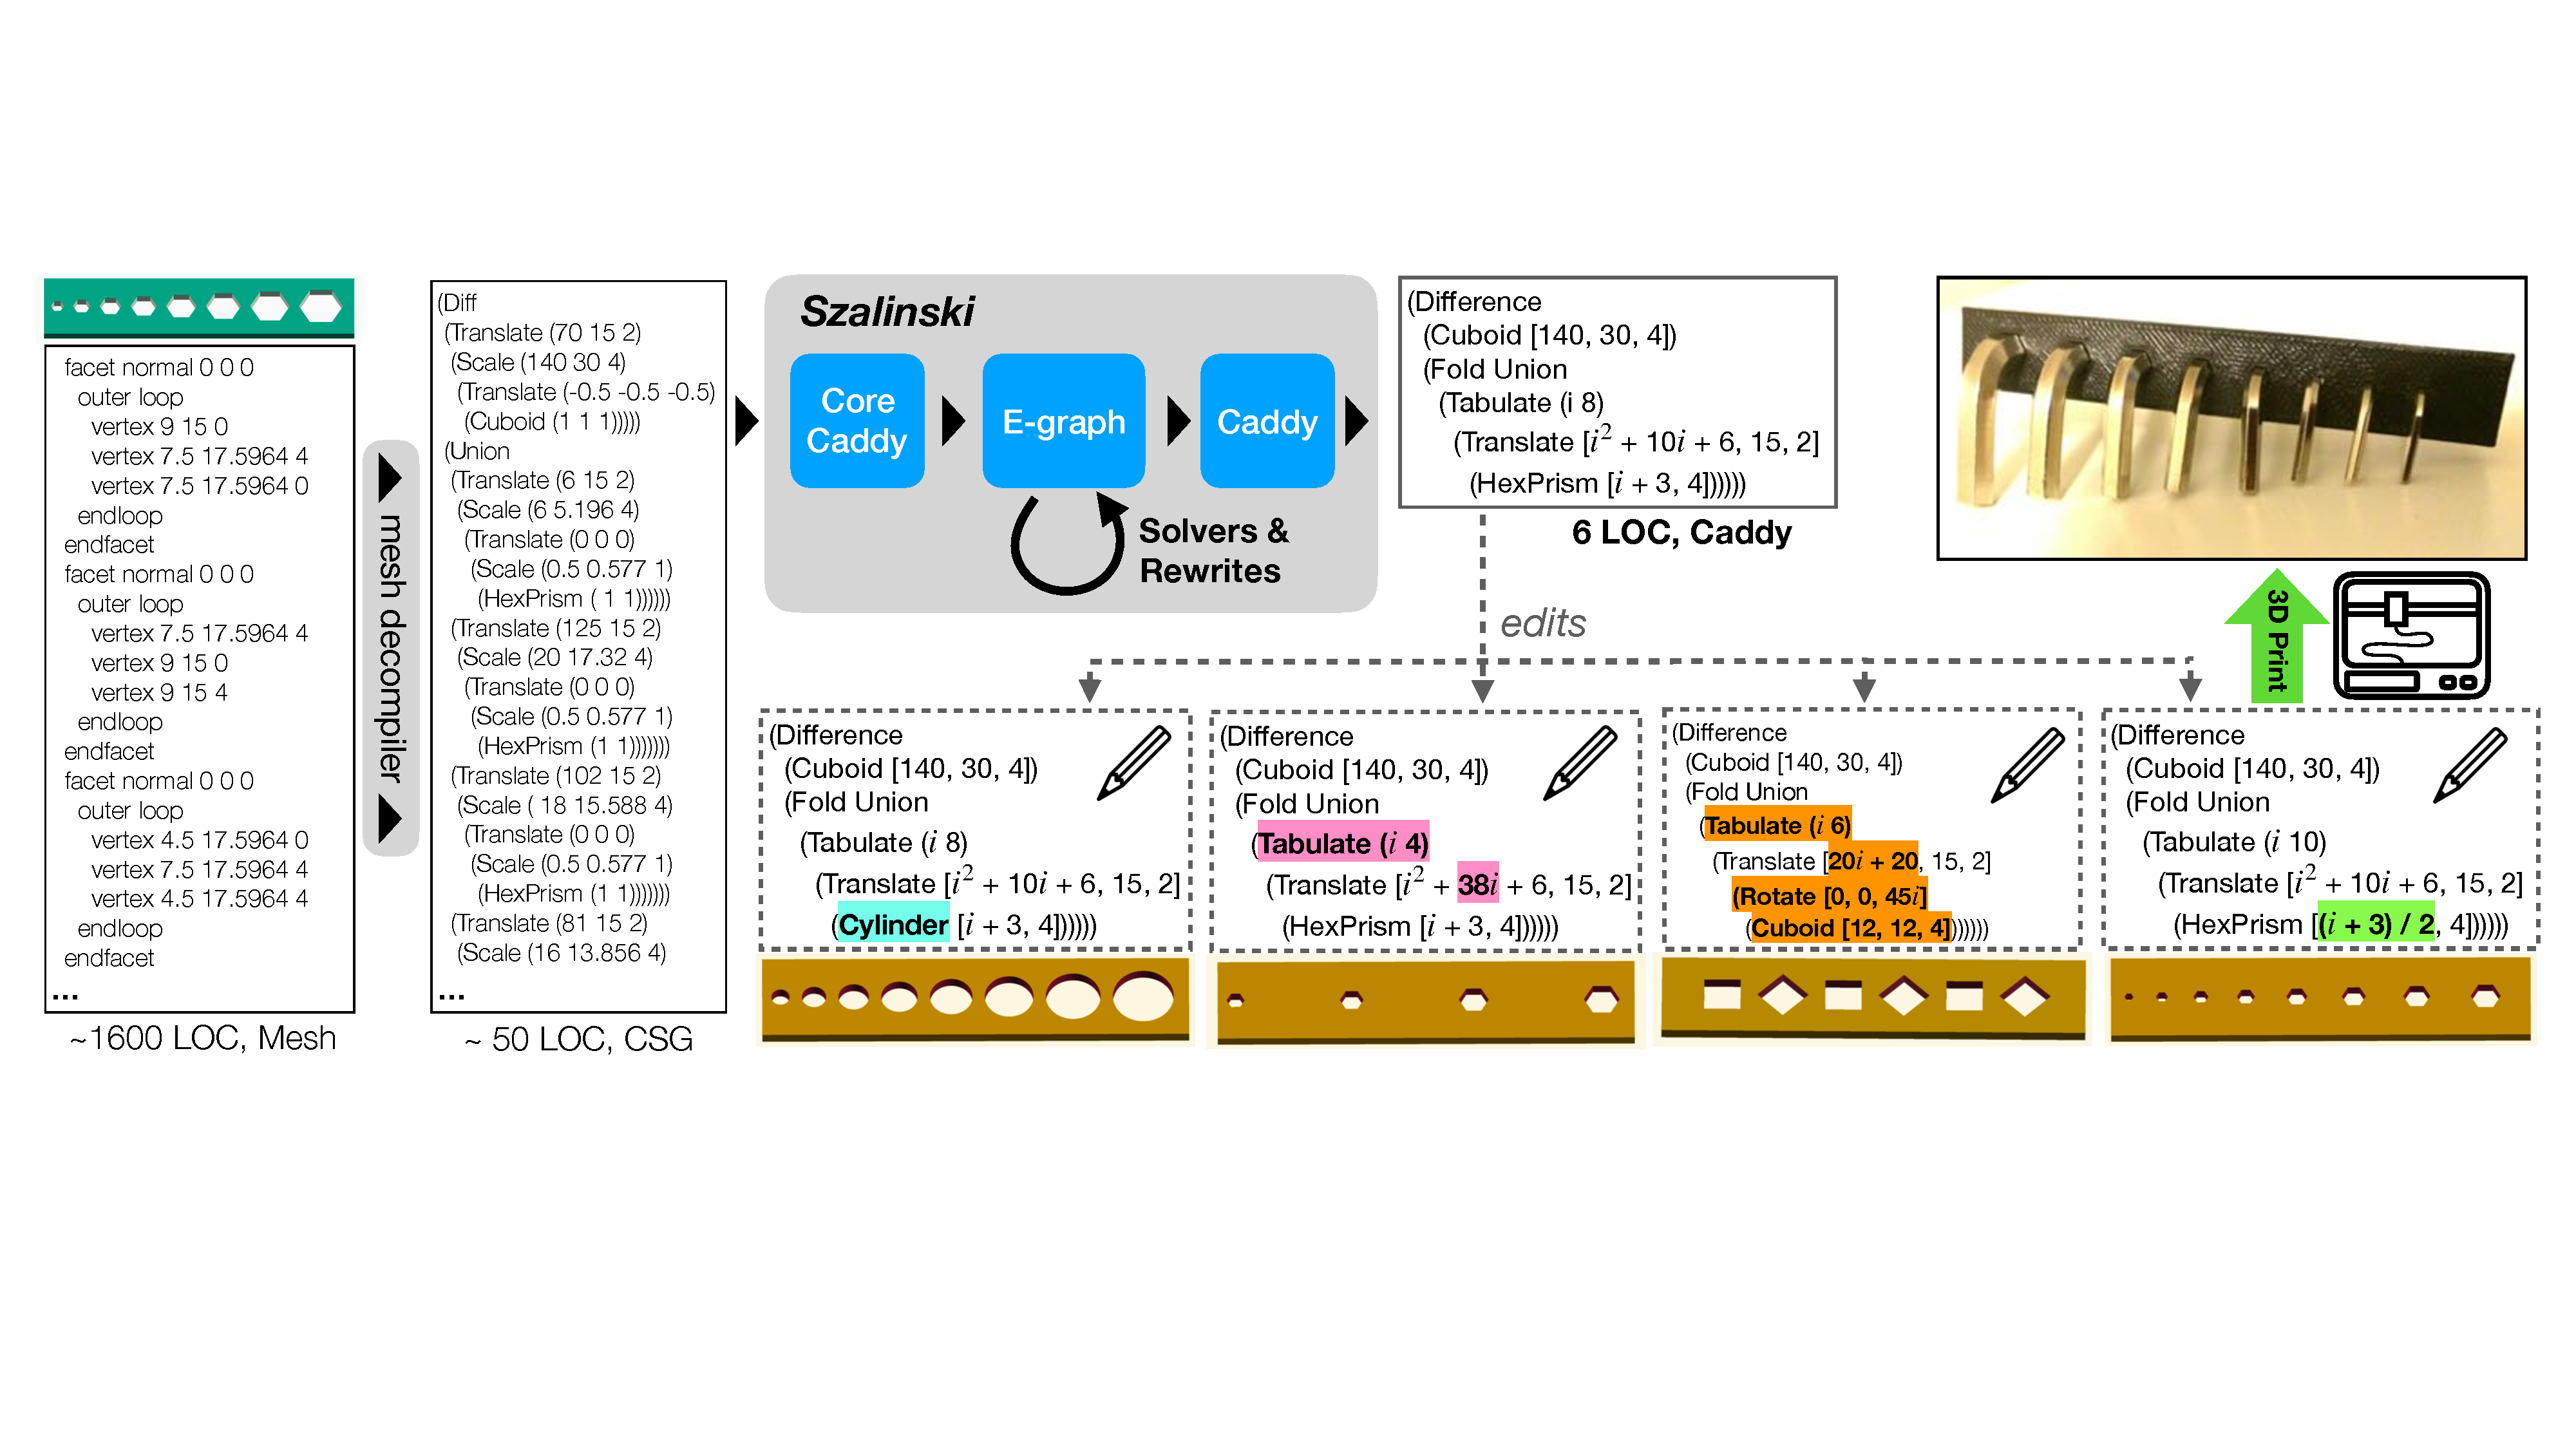
\includegraphics[width=\linewidth]{sz-overview}
  \caption[Szalinski decompiles flat CSG into structured CAD]{
  (图源自 Nandi et.\ al.\ \cite{szalinski})
  现有的网格反编译器(mesh decompiler)将三角网格转换为平面的计算固体几何(CSG)表达式。
  \sz~\cite{szalinski} 在一种称为 Core Caddy 的格式中输入这些 CSG 表达式,
    基于 Caddy 语言综合(synthesizes)了更小的、结构化的程序,它具有函数式编程的特性。 
    % 综合 synthesizes 这个翻译来自于《形式化方法概貌》
    这可以通过简化编辑来简化定制:
      小的、主要是局部更改,来产生有用的不同模型。
    照片展示了定制孔尺寸后 3D 打印的六角扳手架。
    \sz 是基于 \egg 高性能、\eclass 分析和动态重写的可扩展 等式饱和 驱动的。
  }
  \label{fig:sz-overview}
\end{figure}


% Several tools have emerged
%   that reverse engineer high level
%   Computer Aided Design (CAD) models from polygon
%   meshes and voxels~\cite{reincarnate, inverse, shape, csgnet, latex}.
% The output of these tools are constructive solid geometry (CSG) programs.
% A CSG program is comprised of
%   3D solids like cubes, spheres, cylinders,
%   affine transformations like scale, translate, rotate
%   (which take a 3D vector and a CSG expression as arguments),
%   and binary operators like union, intersection, and difference
%   that combine CSG expressions.
% For repetitive models like a gear, CSG programs can be too long
%   and therefore difficult to comprehend.
% A recent tool, \sz~\cite{szalinski},
%   extracts the inherent structure
%   in the CSG outputs of mesh decompilation tools
%   by automatically inferring maps and folds (\autoref{fig:sz-overview}).
% \sz accomplished this using \egg's extensible equality saturation system,
%   allowing it to:
目前已有几种工具可以从多边形网格和体素中逆向 CAD(高级计算机辅助设计,Computer Aided Design)模型
  ~\cite{reincarnate, inverse, shape, csgnet, latex}。
这些工具的输出是构造实体几何(CSG)程序。
一个 CSG 程序由 3D 实体如立方体、球体、圆柱体、仿射变换(如缩放、平移、旋转)
  和二元运算符如并集、交集和差集组成,它们结合了 CSG 表达式。
对于像齿轮这样的重复模型,CSG 程序可能太长,因此难以理解。
一个近来的工具, \sz~\cite{szalinski} ,通过自动推断映射(maps)和折叠(folds)( \autoref{fig:sz-overview})
  ,可以在网格反编译(mesh decompilation)工具的 CSG 输出中提取固有结构。
\sz 通过 \egg 的可扩展 等式饱和 系统实现了这一目标:


\begin{itemize}

  % \item Discover structure using loop rerolling rules.
  %   This allows \sz to infer functional patterns like
  %   \texttt{Fold}, \texttt{Map2}, \texttt{Repeat} and
  %   \texttt{Tabulate} from flat CSG inputs.
  \item 使用循环重投(loop rerolling)规则发现结构。
    这使得\sz 能够从平面CSG输入中推断出
    \texttt{Fold}, \texttt{Map2}, \texttt{Repeat} 和 \texttt{Tabulate} 
    等函数模式。

  % \item Identify equivalence among CAD terms that are
  %   expressed as different expressions by mesh decompilers.
  %   \sz accomplishes this by using CAD identities.
  %   An example of one such CAD identity in \sz is
  %   $e \leftrightarrow \mathit{rotate}~[0 ~ 0 ~ 0] ~ e$.
  %   This implies that any CAD expression $e$
  %   is equivalent to a CAD expression that applies
  %   a rotation by zero degrees about x, y, and z axes
  %   to $e$.
  \item 识别由网格解压器表示为不同表达式的 CAD 术语之间的等价性。
    \sz 通过使用 CAD id (CAD identities)来实现这一点。
    \sz 中的一个 CAD id 示例是
    $e \leftrightarrow \mathit{rotate}~[0 ~ 0 ~ 0] ~ e$。
    这意味着任何 CAD 表达式 $e$ 等价于对 $e$ 应用 x, y, z 轴上零度旋转的 CAD 表达式。

  % \item Use external solvers to
  %   speculatively add potentially profitable
  %   expressions to the \egraph.
  %   Mesh decompilers often generate CSG expressions
  %   that order and/or group list elements in
  %   non-intuitive ways.
  %   To recover structure from such expressions,
  %   a tool like \sz must be able to reorder and regroup
  %   lists that expose any latent structure.
  \item 使用外部求解器向 \egraph 中添加可能有利可图的表达式。
    网格解压器经常生成以非直观方式排序和/或分组列表元素的 CSG 表达式。
    为了从这样的表达式中恢复结构,\sz 这样的工具必须能够重新排序和重新分组列表,暴露任何潜在结构。

\end{itemize}

% \subsubsection{Implementation}
\subsubsection{实现}


% Even though CAD is
%   different from traditional languages
%   targeted by programming language techniques,
%   \egg supports \sz's CAD language in a straightforward manner.
% \sz uses purely syntactic rewrites to express
%   CAD identities and some loop rerolling rules
%   (like inferring a \texttt{Fold} from a list of CAD expressions).
% Critically, however, \sz relies on \egg's
%   dynamic rewrites and \eclass analysis to infer functions
%   for lists.
尽管 CAD 与编程语言技术针对的传统语言不同,但是 \egg 以直接的方式支持 \sz 的 CAD 语言。
\sz 使用纯语法重写来表示 CAD 身份和一些循环重绕规则
  (如从 CAD 表达式列表推断出 \texttt{Fold} )。
然而关键的是,\sz 依赖于 \egg 的动态重写和 \eclass 分析来推断列表的函数。

% 此段翻译未仔细校对
% Consider the flat CSG program in \autoref{fig:sz-egg-input}.
% A structure finding rewrite first rewrites the flat list of \texttt{Union}s to:
% $$\texttt{(Fold Union (Map2 Translate [(0 0 0) (2 0 0) ...] (Repeat Cube 5)))}$$
% The list of vectors is stored as \texttt{Cons} elements (sugared above for brevity).
% \sz uses an \eclass analysis to track the accumulated lists in a similar style
%   to constant folding.
% Then, a dynamic rewrite uses an arithmetic solver to rewrite the concrete
%   list of 3D vectors in the analysis data
%   to \mbox{\texttt{(Tabulate (i 5) (* 2 i))}}.
% A final set of syntactic rewrites can hoist the \texttt{Tabulate}, yielding the
%   result on the right of \autoref{fig:sz-egg}.
% Thanks to the set of syntactic CAD rewrites, this structure finding even works
%   in the face of CAD identities.
% For example, the original program may omit the no-op
%   \texttt{Translate (0 0 0)}, even though it is necessary to see repetitive
%   structure.
考虑 \autoref{fig:sz-egg-input} 中的平面 CSG 程序。
结构发现重写首先将平面的 \texttt{Union} 列表重写为:
$$\texttt{(Fold Union (Map2 Translate [(0 0 0) (2 0 0) ...] (Repeat Cube 5)))}$$
向量列表存储为 \texttt{Cons} 元素(上面简化了)。
\sz 使用 \eclass 分析来跟踪累积列表,类似于常量折叠。
然后,动态重写使用算术求解器重写分析数据中的具体 3D 向量列表,
  以 \mbox{\texttt{(Tabulate (i 5) (* 2 i))}} 的形式。
最后一组语法重写可以提升(hoist) \texttt{Tabulate},得到 \autoref{fig:sz-egg} 右侧的结果。
由于一系列 CAD 语法 重写的存在,即使面对 CAD id,这种结构发现也能正常工作。
例如,原始程序可能省略无操作的 \texttt{Translate (0 0 0)},即使它是观察重复结构所必需的。

\begin{figure}
\begin{subfigure}[b]{0.3\linewidth}
  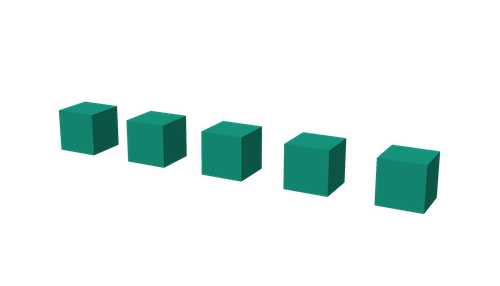
\includegraphics[width=\linewidth]{cubes}
  % \caption{Five cubes in a line.}
  \caption{一条线中的五个立方体。}
\end{subfigure}
\hfill
\begin{subfigure}[b]{0.3\linewidth}
  \begin{lstlisting}[language=Rust, gobble=4, basicstyle=\footnotesize\ttfamily]
    (Union
      (Translate (0 0 0) Cube)
      (Translate (2 0 0) Cube)
      (Translate (4 0 0) Cube)
      (Translate (6 0 0) Cube)
      (Translate (8 0 0) Cube))
  \end{lstlisting}
  % \caption{Flat CSG input to \sz.}
  \caption{Flat CSG 输入到 \sz。}
  \label{fig:sz-egg-input}
\end{subfigure}
\hfill
\begin{subfigure}[b]{0.35\linewidth}
  \begin{lstlisting}[language=Rust, gobble=4, basicstyle=\footnotesize\ttfamily, showlines=true, xleftmargin=5mm]
    (Fold Union
      (Tabulate (i 5)
        (Translate
          ((* 2 i) 0 0)
          Cube)))

  \end{lstlisting}
  % \caption{Output captures the repetition.}
  \caption{输出捕获了重复。}
  \label{fig:sz-egg-output}
\end{subfigure}
  \caption{
    % \sz integrates solvers into \egg's equality saturation as a dynamic rewrite.
    % The solver-backed rewrites can transform repetitive lists into
    % \texttt{Tabulate} expressions that capture the repetitive structure.
    \sz 将求解器作为动态重写集成到 \egg 的 等式饱和 中。
    支持求解器的重写可以将重复列表转换为捕获重复结构的 \texttt{Tabulate} 表达式。%?solver-backed
  }
  \label{fig:sz-egg}
\end{figure}


% In many cases, the repetitive structure of input CSG expression is further
%   obfuscated because subexpressions may appear in arbitrary order.
% For these inputs, the arithmetic solvers must first reorder
%   the expressions to find a closed form like a \texttt{Tabulate}
%   as shown in \autoref{fig:sz-egg}.
% However, reordering a list does not preserve equivalence, so adding it to the
%   \eclass of the concrete list would be unsound.
% \sz therefore introduces \textit{inverse transformations},
%   a novel technique that allows solvers to speculatively reorder and regroup list
%   elements to find a closed form.
% The solvers annotate the potentially profitable expression with the
%   permutation or grouping that led to the successful discovery
%   of the closed form.
% Later in the rewriting process, syntactic rewrites eliminate the inverse
%   transformations when possible
%   (e.g., reordering lists under a \texttt{Fold Union} can be eliminated).
% \egg supported this novel technique without modification.
在很多情况下,输入 CSG 表达式的重复结构进一步混淆,因为子表达式可能以任意顺序出现。
对于这些输入,算术求解器必须首先重新排序表达式,以找到像 \texttt{Tabulate} 这样的封闭形式,如 \autoref{fig:sz-egg} 所示。然
而,重新排序列表不会保留等价性,因此将其添加到具体列表的 \eclass 中将是不安全的。
因此,\sz 引入了新技术 \textit{反向变换(inverse transformations)},
  允许求解器推测重新排序和重新分组列表元素以找到封闭形式。求解器使用导致成功发现封闭形式的排列或分组注释可能有利可图的表达式。
在重写过程的后期,语法重写在可能时删除反向变换
  (例如,在\texttt{Fold Union} 下重新排序列表可以被删除)。
\egg 支持了这种新颖的技术,而无需修改。

% \subsubsection{Results}
\subsubsection{评估}

% \sz's initial protoype used a custom \egraph written in OCaml.
% Anecdotally, switching to \egg
%   removed most of the code,
%   eliminated bugs,
%   facilitated the key contributions of solver-backed rewrites and inverse transformations,
%   and made the tool about $1000 \times$ faster.
% \egg's performance allowed a shift from running on small, hand-picked
%   examples to a comprehensive evaluation on over 2000 real-world models from
%   a 3D model sharing forum~\cite{szalinski}.
\sz 的初始原型使用 OCaml 编写的自定义 \egraph。
有趣的是,使用 \egg 删除了大部分代码,
  消除了错误,
  促进了求解器支持的重写(solver-backed rewrites)和反向变换(inverse transformations)
  的关键贡献, 
  并使工具快了约 $1000 \times$。
\egg 的性能允许从运行小型手工选择的示例转变为对来自 3D 模型共享论坛~\cite{szalinski}
  的 2000 多个真实世界模型的综合评估。


%%% Local Variables:
%%% TeX-master: "egg"
%%% End:
